\begin{frame}[allowframebreaks]
  \frametitle{Path Integral Isomorphism}
  For a single particle moving in one spatial dimension potential
  \footnote[frame]{
   ``Statistical Mechanics: Theory and Molecular Simulation'', Mark E. Tuckerman 
  }
  $$
  \hamil = \frac{\hat{p}^2}{2m} + \hat{V}(\hat{x}) \equiv \hat{T} + \hat{V}
  $$
  The quantum partition function
  \begin{align*}
    \label{eq:quantum_partition_function}
    Z &= \tr\left[e^{-\beta\hamil}\right]
        = \tr\left[(e^{-{\beta\over P}\hamil})^P\right]
        = \tr\left[(e^{-{\beta_P}\hamil})^P\right]
        % \qquad\qquad \beta_P = {\beta\over P}
        \cr
    &= \int\dt{x_1}\,
      \braket{ x_1| (e^{-\beta_P\hamil})^P | x_1} \cr
    &= \int\dt{x_1}\ldots\int\dt{x_P}\,
      \braket{ x_1| e^{-\beta_P\hamil} | x_2}
      \ldots
      \braket{ x_P| e^{-\beta_P\hamil} | x_1}
  \end{align*}
  Note the connection between the quantum propagator and the density matrix,
  \begin{equation*}
    \label{eq:density_mat_and_propagator}
    \braket{ x'| e^{-i\hamil t/\hbar} | x}
    % \qquad\Rightarrow\qquad
    \qquad
    \tikz \draw [->, >=stealth, blue, line width=0.5pt] (0, 0) -- node[above,
    midway]{$t \to \tau= i\beta\hbar$} (2.5, 0.0);
    \qquad
    \braket{ x'| e^{-\beta\hamil} | x}
    % ;\quad t = -i\beta\hbar
  \end{equation*}
  Hence the name \emph{imaginary-time path integral}. By using the Trotter splitting\footnote[frame]{
    There are higher-order splitting techniques.
  }
  \begin{align*}
    e^{-\beta_P\hamil} &=
    e^{-\beta_p\hat{V}/2}e^{-\beta_p\hat{T}}e^{-\beta_p\hat{V}/2} +
    {\cal O}(\beta_P^3) \cr
    \Rightarrow \quad \braket{ x_i| e^{-\beta_P\hamil} | x_j} &\approx
    \left(m \over2\pi\beta_P\hbar^2\right)^{1/2}\,
    e^{
      -\beta_P
      \left[
         {m\over2(\beta_P\hbar)^2} (x_i - x_j)^2
                                                          + 
        {1\over2} \bigl(V(x_i) + V(x_j)\bigr)
      \right]
    }
  \end{align*}
  % \pagebreak
  % \begin{equation*}
  %   e^{-\beta_P\hamil} =
  %   e^{-\beta_p\hat{V}/2}e^{-\beta_p\hat{T}}e^{-\beta_p\hat{V}/2} + \textrm{O}(\beta_P^3)
  % \end{equation*}
  % \begin{equation*}
  %   \braket{ x_i| e^{-\beta_P\hamil} | x_j} \approx
  %   \left(m \over2\pi\beta_P\hbar^2\right)^{1/2}\,
  %   e^{
  %     -\beta_P
  %     \left[
  %       {1\over2} \bigl(V(x_i) + V(x_j)\bigr) + 
  %        {m\over2(\beta_P\hbar)^2} (x_i - x_j)^2
  %     \right]
  %   }
  % \end{equation*}
  
  \begin{align*}
    Z &= \tr\left[e^{-\beta\hamil}\right] \cr
      &=\lim_{P\to\infty} 
        \int\dt{x_1}\ldots\int\dt{x_P}\,
        \left(m \over2\pi\beta_P\hbar^2\right)^{P/2}
        \exp\Biggl\{
          \displaystyle
          -\beta_P
          \underbrace{
          \sum_{i=1}^P \left[
            {m\over2(\beta_P\hbar)^2} (x_{\tikzmark{ring_polymer_bc} i+1} - x_i)^2
            +
            V(x_i)
        \right]
        }_{V_{\text{eff}}(x_1,\ldots,x_P)}
        \Biggr\} \Bigg|_{x_{P+1} = x_1}
  \end{align*}

  % \begin{tikzpicture}
  %   [overlay, remember picture]
  %   \node[
  %   draw=red, rounded corners=3pt, above right = 3em and 0em of
  %   ring_polymer_bc, text width=1.2cm, align=center, % inner sep=0pt
  %   ] (rp_bc_note) {
  %     \small $x_{P+1} = x_1$
  %   };                     
  %   \draw[red,->, >=stealth, in=90, out=-90] (rp_bc_note.south) to ($
  %   (ring_polymer_bc.north east) + (6pt, 6pt)$);
  % \end{tikzpicture}

  \begin{figure}
  \centering
  \resizebox{0.60\textwidth}{!}{
  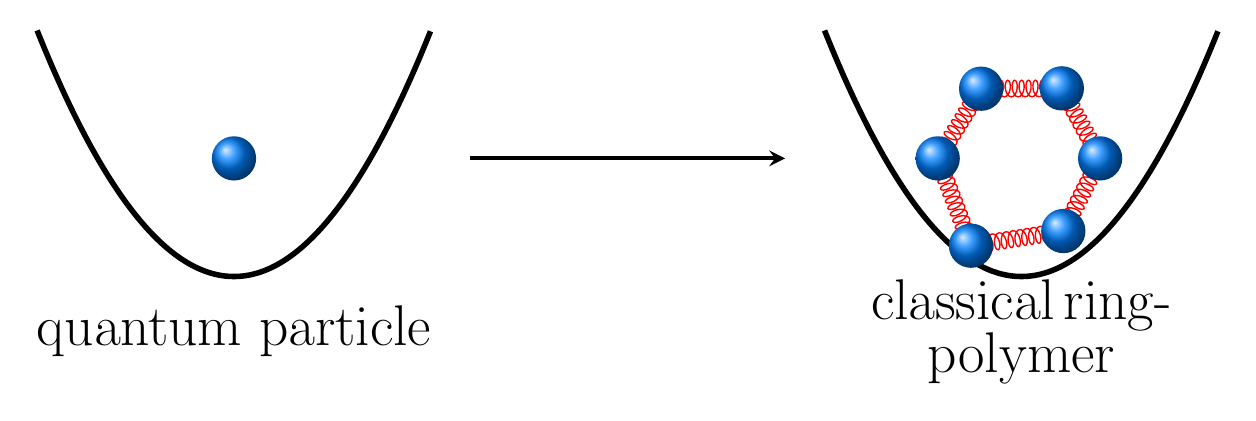
\begin{tikzpicture}
    [
    spring/.style={
      line width=0.5pt, decorate,
      decoration={
        coil, amplitude=3.0, 
        segment length=2.5
      }}, 
    potential/.style={
      line width=0.5pt, decorate,
      color=green!50!black,
      decoration={
        snake, amplitude=2.0, 
        segment length=100
    }}
    ]
    \def\pointsA{
          1.0000/   0.0000,
          0.5136/   0.8896,
         -0.5112/   0.8853,
         -1.0629/   0.0000,
         -0.6401/  -1.1086,
          0.5326/  -0.9226
    }
    \def\rpoffset{(4.0, -0.5)}

     % Draw the potential
     \draw [line width=2pt, domain=-12.5:-7.5] plot [samples=300] (\x, {0.5 * (\x + 10) * (\x + 10) - 1.5});
     \draw [line width=2pt, domain=-2.5:2.5] plot [samples=300] (\x, {0.5 * (\x + 0) * (\x + 0) - 1.5});
     % Draw an arrow
     \draw [line width=1.5pt, ->, >=stealth] (-7, 0) -- (-3, 0);

    % First, draw the springs for the first RP
    \draw[spring, color=red] (  1.0000,   0.0000) 
                          -- (  0.5136,   0.8896) 
                          -- ( -0.5112,   0.8853) 
                          -- ( -1.0629,   0.0000) 
                          -- ( -0.6401,  -1.1086) 
                          -- (  0.5326,  -0.9226) 
                          -- cycle;
    % % First, draw the springs for the second RP
    % \draw[spring, color=blue] ($ (  1.0000,   0.0000) + (4.0, -0.5) $)
    %                       -- ($ (  0.5136,   0.8896) + (4.0, -0.5) $)
    %                       -- ($ ( -0.5112,   0.8853) + (4.0, -0.5) $)
    %                       -- ($ ( -1.0629,   0.0000) + (4.0, -0.5) $)
    %                       -- ($ ( -0.6401,  -1.1086) + (4.0, -0.5) $)
    %                       -- ($ (  0.5326,  -0.9226) + (4.0, -0.5) $)
    %                       -- cycle;

    % Draw the single particles
    \shade[shading=ball, ball color=blue!50!cyan] (-10, 0) circle (8pt);

    \foreach \x/\y in \pointsA {
      \coordinate (A) at (\x, \y);
      % draw the interaction between the two atoms
      % \draw[potential] (A) -- ++\rpoffset;
      % Ring-Polymer of the first atom
      \shade[shading=ball, ball color=blue!50!cyan] (A) circle (8pt);
      % Ring-Polymer of the second atom
      % \shade[shading=ball, ball color=red!50!pink] ($ (A) + (4.0, -0.5) $) circle (8pt);
    }
    \node[] at (-10, -2.2) {
      % \fontsize{24}{12pt}\selectfont
      \huge
      % $Z = \tr \left[e^{-\beta\hamil}\right]$
      quantum particle
    };
    \node[text width=5cm, align=center] at (0.0, -2.2) {
      % \fontsize{24}{12pt}\selectfont
      \huge
      % configuration integral of classical ring-polymer
      classical ring-polymer
    };
  \end{tikzpicture}}
\end{figure}
  \begin{itemize}
    \item Maps the \emph{quantum partition function} to the \emph{configuration integral} of 
      classical ring-polymers.
    \item \emph{EXACT} when $P \to \infty$. Reduce to classical partition function when $P = 1$.
    % \item When there are multiple nuclei, indistinguishability of identical nuclei is \emph{neglected}!
    \item The integral can be sampled with Monte Carlo method (PIMC, not
      covered in this talk), but for MD
    we need \emph{momenta}!
  \end{itemize}
\end{frame}

%%% Local Variables:
%%% mode: latex
%%% TeX-master: t
%%% End:
